\documentclass[a4paper,twoside]{article}

\usepackage{graphicx}
\usepackage{subfigure}
\usepackage{calc}
\usepackage{amssymb}
\usepackage{amstext}
\usepackage{amsmath}
\usepackage{amsthm}
\usepackage{multicol}
\usepackage{pslatex}
\usepackage{apalike}
\usepackage{SCITEPRESS}
\usepackage[small]{caption}
\graphicspath{{images/}}

\subfigtopskip=0pt
\subfigcapskip=0pt
\subfigbottomskip=0pt

\begin{document}

\title{Evaluating Artificial Neural Networks and Traditional Approaches for Risk Analysis in Software Project Management \subtitle{A case study with PERIL dataset} }

\author{\authorname{Carlos H. M. S. Timoteo\sup{1}, Meuser J. S. Valenca\sup{1} and Sergio M. M. Fernandes\sup{1}}
\affiliation{\sup{1}Computer Engineering Department, University of Pernambuco, Rua Benfica, Recife, Brazil}
\email{\{chmst, mjsv, smurilo\}@ecomp.poli.br}
}

%The paper must have at least one keyword. The text must be set to 9-point font size and without the use of bold or italic font style. For more than one keyword, please use a comma as a separator. Keywords must be titlecased.
\keywords{Software Project, Risk Management, Risk Analysis, Support Vector Machine, MultiLayer Perceptron, Monte Carlo Simulation, Linear Regression Model}

%The abstract should summarize the contents of the paper and should contain at least 70 and at most 200 words. The text must be set to 9-point font size.
\abstract{Many software project management end in failure. Risk analysis is an essential process to support project success. There is a growing need for systematic methods to supplement expert judgment in order to increase the accuracy in the prediction of risk likelihood and impact. In this paper, we evaluated support vector machine (SVM), multilayer perceptron (MLP), a linear regression model and monte carlo simulation to perform risk analysis based on PERIL data. We have conducted a statistical experiment to determine which is a more accurate method in risk impact estimation. Our experimental results showed that artificial neural network methods proposed in this study outperformed both linear regression and monte carlo simulation.}

\onecolumn \maketitle \normalsize \vfill

\section{\uppercase{Introduction}}
\label{sec:introduction}

%Apresentar a estatística da quantidade de projetos de software que falham.
\noindent How risky are software projects? Several studies about effectiveness of software cost, scope, schedule estimation techniques; surveys from software professionals in industry; and analysis of project portfolios have been done to answer this question \cite{budzier2013double}. However, there is not a consensus. 

Some remarkable work support that software projects involve risky activities. \cite{schmidt2001identifying} have noticed that many software development projects end in failure. They showed that around twenty five percent of all software projects are canceled outright and as many as eighty percent of all software projects run over their budget, exceeding it by fifty percent in average. \cite{bannerman2008risk} states that industry surveys suggest that only a quarter of software projects succeed outright, and billions of dollars are lost annually through project failures or projects that do not deliver promised benefits. Moreover, \cite{bannerman2008risk} shows evidences that it's a global issue, impacting private and public sector organizations.

%Apresentar a definição de risco (PMBOK). As características do risco de projeto (estocásticos pois levam em consideração o instante atual, podem estar interrelacionados casualmente, a previsão pode ser bem baseada em dados históricos).
\cite{BOEHM1991} defined risk as the possibility of loss or injury. This definition can be expressed by risk exposure formula. Even Boehm cites risk exposure as the most effective technique for risk priorization after risk analysis, \cite{bannerman2008risk} considers this definition limited and unsuitable. In classical decision theory, risk was viewed as reflecting variation in the probability distribution of possible outcomes, whether negative or positive, associated with a particular decision. This study takes into account PMI \cite{PMBOK2008} definition whereupon project risk is a certain event or condition that, if it occurs, has a positive or negative effect on one or more project objectives. A complementary definition proposed by Haimes \cite{haimes2011risk} is also considered, which express risk as a measure of the probability and severity of adverse effects.

A risk factor is a variable associated with the occurrence of an unexpected event. Risk factors are correlational, not necessarily causal and, if one of them occurs, it may have one or more impacts. According to \cite{haimes2011risk}, risks can often arise as the result of an underlying stochastic process occurring over time and space, but also, can occur based on deterministic risk factors. Risk estimation can be achieved based on historical information and knowledge from previous similar projects and from other information sources \cite{PMBOK2008}. 

%Páragrafo de ligação para os problemas
Recent perceptions about risk management and the inherent challenges posed by the nature of software projects contributes to the lack of project stability from majority of software project organizations \cite{kwak2004project}. \cite{kwak2000calculating} identified risk management as the least practiced discipline among different project management knowledge areas. The authors mention that, probably, a cause for it is that software developers and project managers perceive managing uncertainty processes and activities as extra work and expense.

%Apresentar o problema na análise de risco devido a ausencia de dados históricos em se tratando de projetos. Falta de repetibilidade das atividades. A dificuldade em estimar de forma precisa a probabilidade e o impacto dos riscos.
A difficult task in risk analysis is to perform accurate estimates of the probability and impact associated with an unexpected outcome \cite{BOEHM1991}. \cite{bannerman2008risk} have found a limitation on Boehm's definition - it is very difficult, in practice, to estimate the probability of many risk factors, especially in software projects. Probability and impact can only be meaningfully determined for activities that are repeated many times, under controlled circumstances. The one-off nature of many software project activities mitigates accurate estimates.

%Apresentar o problema da falta de uma ferramenta para suportar gestores que utilizam a intuição ao invés da lógica para analisar o risco.
The need to manage risks (undesired events) increases exponentially with system complexity. Managing those events in such complex systems becomes difficult to identify and predict undesirable expected or unexpected events occurrence because of huge amount of risk factors involved and their relations. There is an increasing need for more systematic methods and tools to supplement individual knowledge, judgment, and experience. These human traits are often sufficient to address less complex and isolated risks. For example, a portion of the most serious issues encountered in system acquisition are the result of risks that are ignored, due to its low likelihood, until they have already created serious consequences \cite{higuera1996software}.

%Justificar a escolha dos métodos analisados nesse estudo.
The Guide to the Project Management Body of Knowledgment \cite{PMBOK2008} presents Monte Carlo Simulation as a good practice method to project risk analysis. However, there are some limitations in the adoption of this approach that makes it unfeasible \cite{Ibbotson2005}. Simulations can lead to misleading result if inappropriate inputs, derived from subjective parametrization, are entered into the model. Commonly, the user should be prepared to make the necessary adjustments if the results that are generated seem out of line. Moreover, Monte Carlo can not model risks correlations. That means the numbers coming out in each draw are random and in consequence, an outcome can vary from its lowest value, in one period, to the highest in the next. Therefore, alternative approaches must be considered to predict risk likelihood and impact, taking into account project risk characteristics and Monte Carlo Simulation limitations. Thus, risk analysis should be a more accurate and easier task, from users point of view.

%Apresentar o objetivo desse trabalho: Analisar qual abordagem é mais eficiente para a análise do impacto do risco no gerenciamento de projetos de software: redes neurais artificiais ou a abordagem tradicional baseada em simulação de monte carlo. Como base de comparação, será utilizada a regressão linear.
The main purpose of this paper is to analyze which is a more efficient approach to software project risk analysis: Monte Carlo Simulation (MCS) technique or Artificial Neural Networks (ANN's) alternatives through Multilayer Perceptron (MLP) and Support Vector Machine (SVM) related to improved accuracy and decreased error prone. A Linear Regression Model (LRM) is also considered as baseline to evaluation methodology.

%Apresentar a metodologia a ser utilizada nesse estudo. Um experimento estatístico para avaliação do erro de previsão do impacto de riscos obtidos a partir da base de dados do PERIL. As quatro técnicas selecionadas nesse estudo irão prever the outcomes to risk impacts, o erro médio absoluto será calculado thirty times, e um teste de hipótese pode ser necessário para afirmar qual a melhor técnica that fits this dataset.
In summary, the methodology adopted in this study is a statistical experiment to evaluate the prediction error of risk impact from PERIL dataset \cite{kendrick2003identifying}, a framework to identify risks in software project management. The four selected techniques will estimate the outcome to risk impacts. Mean Absolute Error (MAE) will be calculated thirty times for each approach, and then a hypothesis test may be necessary to assert what is a more efficient method that fits this data.

%Apresentar as seções seguintes do trabalho.
In Section \ref{sec:stateofart} is presented project risk management, risk analysis concepts and the chosen techniques used in the experiment. Section \ref{sec:methodology} presents the methodology for this study, including dataset and tools presentation. Section \ref{sec:resultanalysis} presents the result analysis and establishes the best analyzed technique. In the end, Section \ref{sec:conclusion} concludes this work and presents limitations and future works.

\section{\uppercase{State of Art}}
\label{sec:stateofart}

\subsection{Related Work}
%Apresentar trabalhos relacionados a este. Trabalhos que utilizam as mesma técnicas ou técnicas de mesma classe para tratar os mesmo problema.

\noindent After a short bibliographic revision, we have identified in academia that numerous approaches were exploited in risk analysis, that includes Logistic Regression Model (LRM), Bayesian Belief Network (BBN), Artificial Neural Network (ANN), Discriminant Analysis (DA), Decision Tree (DT), Genetic Algorithm (GA), Particle Swarm Optimization (PSO), Fuzzy Set Theory (FST), Neuro-Fuzzy System (NFS), Extended Fuzzy Cognitive Maps (E-FCM), etc.
%\cite{mizuno2001prediction} \cite{huang2004neuro} \cite{hu2007software} \cite{attarzadeh2010novel} \cite{dzega2010classification} \cite{yu2011software} \cite{saxena2012software} \cite{dan2013improving}.

\cite{hu2007software} proposed a method to analyze software risks and predict outcomes of software projects. Genetic algorithm could be utilized as an optimization method to improve ANN in many ways, including weights, network structure and rule learning. The standard ANN was enhanced by introducing GA, in that study. Results of the experiments showed that after introducing GA to the ANN training process, the enhanced software risk evaluation model could be improved notably and achieve higher accuracy when compared to the SVM model. \cite{dan2013improving} proposed an artificial neural network (ANN) prediction model that incorporates with Constructive Cost Model (COCOMO) which was improved by applying PSO, to provide a method which can estimate the software develop effort accurately. \cite{attarzadeh2010novel} utilized ANN to improve accuracy of effort estimation compared to the traditional COCOMO model. \cite{huang2004neuro} have presented a general framework for software estimation based on NFS, the authors improved cost estimation for COCOMO'81.

\cite{yu2011software} showed up a model based on the fuzzy theory. It overcame the difficulty of qualitative indicators and quantitative assessment in the traditional analysis methods. In addition, \cite{saxena2012software} explored neuro-fuzzy techniques to design a suitable model to utilize improved estimation of software effort for NASA software projects. Results showed that NFS has the lowest prediction error compared with existing models. Meanwhile, \cite{lazzerini2011analyzing} suggested a framework to analyze risks using E-FCMs and extended E-FCMs themselves by introducing a special graphical representation for risk analysis.

\cite{mizuno2001prediction} have proposed a new prediction method for risky software projects. The authors have used the logistic regression model to predict whether a project becomes risky or not. However, the proposed estimating approaches for the cost and the duration do not have absolutely high level of accuracy.

\cite{dzega2010classification} have presented results of risk analysis experiments performed using data mining classifiers such as C4.5, RandomTree and Classification and Regression Tree (CART) algorithms. Besides that, they described how boosting and bagging metaclassifiers were applied to improve the results and also analyzed influence of their parameters on generalization abilities in prediction accuracy. Due to a large number of unordered labeled attributes in datasets, MLP and SVM were rejected at early stages, producing low accuracy for each dataset.

In summary, some of those studies proposed methods to software project cost, schedule and effort estimation; another studies proposed approaches to risk classification and software project classification (success, challenged and failed). Moreover, the remainder presented techniques to risk impact estimation on software project management \cite{yu2011software} \cite{saxena2012software} \cite{lazzerini2011analyzing} \cite{dzega2010classification}.

\subsection{Project Risk Management}

%Apresentar a teoria de gerenciamento de risco de projetos (PMBOK). %O objetivo do gerenciamento de riscos. 
\noindent According to \cite{PMBOK2008}, Project Risk Management includes process as planning, identification, analysis, response planning, monitoring and controlling risks of a project. Its purpose is to increase likelihood and impact of positive events and reduce probability and severity of negative events. From management point of view, making informed decisions by consciously assessing what can go wrong, as well as its likelihood and severity of the impact, is at the heart of risk management. This activity involves the evaluation of the trade-offs associated with all policy options for risk mitigation in terms of their costs, benefits, risks and the evaluation of the impact of current decisions on future options.

%O processo de gerenciamento de riscos
A summary of project risk management processes are the following:
\begin{itemize}
\item Planning risk management: The process of defining how conduct risk management activities in a project;
\item Identifying risks: The process of determining risks that can affect project and documenting its characteristics;
\item Performing qualitative risk analysis: The process of prioritizing risks to analyze or additional actions through assessment and combination of its occurrence probability and impact;
\item Performing quantitative risk analysis: The process of analyzing numerically the effect of previous identified risks, in terms of general project objectives;
\item Planning risk responses: The process of developing options and actions to increase opportunities and decrease threats to project objetives;
\item Monitoring and controlling risks: The process of implementing risk responses planning, tracking identified risks, monitoring residual risks, identifying new risks and assessing the efficacy of risk treatment process during the whole project.
\end{itemize}

\subsubsection{Risk Analysis}

% Apresentar o conceito de análise de riscos.
\noindent Analysis is the conversion of risk data into risk decision-making information. Analysis provides the basis for the project manager to work on the "right" and most critical risks. \cite{BOEHM1991} defines risk analysis objective as the assessment of the loss probability and loss magnitude for each identified risk item, and it assess compound risks in risk-item interactions. Typical techniques include performance and cost models, network analysis, statistical decision analysis and quality-factor (such as reliability, availability, and security) analysis.

% Apresentar o processo de análise de riscos. Mostrar que ele é dividido em análise qualitativa e quantitativa.
Risk analysis depends on a good mechanism to identify risks. However, most of the methods assume that managers have the required experience to be aware of all pertinent risk factors, but it can not be the situation. Moreover, many of these methods can be time-consuming and thus too costly to use on a regular basis. Therefore, one popular method for identifying risk factors has been the use of checklists. Unfortunately, these checklists are based in small samples or, even worse, flawed in their risk historical data collection methods.

% Apresentar as técnicas utilizadas no PMBOK para a análise de risco (PRAM)
Most used techniques to risk analysis include \cite{PMBOK2008}:
\begin{itemize}
\item Sensibility analysis: it helps to determine which risks have the higher potential impact on the project. A typical representation of the sensitivity analysis is the tornado diagram;
\item Earned Monetary Value (EMV): it is a statistical concept that computes the average score when the future includes scenarios that may or may not occur (ie, under uncertainty analysis). A common use of this kind of technique is the decision tree analysis;
\item Modeling and simulation: Simulation utilizes a model that converts the detailed specified uncertainties in their potential impact on project objectives. The general iterative simulations are performed using MCS;
\item Specialized opinion: expert judgment (ideally by specialists with relevant and recent expertise) is required to identify the potential impacts on cost and schedule, to assess the likelihood, but also to define input variables and which tools to use.
\end{itemize}

\subsubsection{Monte Carlo Simulation}

% Apresentar a definição da simulação de monte carlo.
\noindent Monte Carlo simulation is a technique that computes or iterates the project cost or schedule many times using input values selected at random from probability distributions of possible costs or durations, to calculate a distribution of possible total project cost or completion dates. \cite{PMBOK2008}.

A model is developed, and it contains certain input variables. These variables have different possible values, represented by a probability distribution function of the values for each variable. The Monte Carlo method is a detailed simulation approach through intensive computing to determine the likelihood of possible outcomes of a project goal; for example, the completion date or total cost. The inputs of the procedure are obtained randomly from specific intervals with probability distribution functions for the durations of schedule activities or items from cost baseline. Those different input values are used to construct a histogram of possible results to the project and its relative probability, but also the cumulative probability to calculate desired contingency reserves for time or cost. Additional results include the relative importance of each input in determining the overall project cost and schedule \cite{kwak2007exploring}.

\subsection{Artificial Neural Networks}

\noindent An Artificial Neural network (ANN) is a massively parallel distributed processor made up of simple processing units, which has a natural propensity \cite{linlee1996neuralfuzzy}. It adopts non-parametric regression estimates made up of a number of interconnected processing elements between input and output data. They have excellent learning and generalizing capabilities.


\subsubsection{MultiLayer Perceptron}

% Apresentar a definição de MLP.
\noindent MLP model is constituted of some neurons organized in at least three layers. The first of them is the input layer, in which input variables are directly connected to a exclusive neuron. The next is the hidden layer that completely connects the neurons from previous layer to the neurons in output layer. Lastly, output layer represents ANN outcome. Each input in a neuron has an associated weight to be adjusted by training algorithm. A common MLP model contains a bias neuron. The MLP is a direct graph, in which inputs data are propagated from input layer to hidden layer\(s\) and from hidden layer to the output layer. The data flow in forward path in a MLP is known as "forward phase". The data flow in opposite way is the "backward phase".

One major concern of ANN is the stability-plasticity dilemma. Although continuous learning is desired in ANN, further learning will cause the ANN to lose its memory when the weights have reached a steady state \cite{haykin1994neural}. The Backpropagation algorithm is used as the training method because it allow us to adjust weights of multilayer networks, towards Generalized Delta Rule \cite{rumelhart1985learning}. 

\subsubsection{Support Vector Machine}

% Apresentar a definição de SVM.
\noindent Support Vector Machine (SVM) is an elegant tool for solving pattern recognition and regression problems. It has attracted a lot of attention from researchers due to its ability to provide excellent generalization performance. The goal of SVM regression is to estimate a function that is as "close" as possible to the target outcomes for every input data in training set and at the same time, is as "flat" as possible for good generalization. More details about SVM can be found in \cite{Shevade1999}.
%Let $x$ denote the input vector of the SVM and $z$ to denote the feature space vector which is related to $x$ by a transformation, $z = \phi(x)$. Let the training set, ${x_i, d_i}$, consists of $m$ data points where $x_i$ is the $i$-th input pattern and $d_i$ is the corresponding target value, $d_i \in \mathbb{R}$. 
%\begin{equation}\label{eq_f}
%    f(x)= \omega \bullet \phi(x) + b
%\end{equation}
% Apresentar alguns trabalhos que utilizam essa técnica, o método e os resultados obtidos.
%\subsection{Multiple Linear Regression}
% Apresentar a definição da regressão linear.
%\noindent Multiple Linear Regression is among the most used statistical data analysis techniques. These models obtain an additive function relating a target variable to a set of predictor variables. This additive function is a sum of elements of the formula $\beta_i \times X_i$, where $X_i$ is a predictor variable matrix and $\beta_i$ is the weight matrix in the multiple linear regression \cite{torgo2003data}.

\section{\uppercase{Methodology}}
\label{sec:methodology}
% Apresentar o objetivo do estudo. Justificar a escolha e a necessidade da base de dados, do pre processamento dos dados, do uso de ferramentas e os experimentos a serem conduzidos.

\noindent In this paper, we analyzed which is a more efficient approach to risk analysis of software projects: Monte Carlo Simulation, Multilayer Perceptron, Support Vector Machine or a Linear Regression Model. The Linear Regression Model was considered as baseline approach. The analysis was made in terms of prediction accuracy. Accuracy means the degree of closeness of a predicted outcome to the true value. A metric of accuracy is the Mean Absolute Error (MAE) given by

\begin{equation}\label{eq_MAE}
    MAE=\frac{1}{n}\sum_{i=1}^{n} |e_i|,
\end{equation}
where $e_i=f_i - y_i$, $f_i$ is the calculated outcome, $y_i$ is the expected outcome and $n$ is the number of data pairs.

The four selected techniques have predicted the outcome to risk impacts. Mean Absolute Error was calculated thirty times for each method. Nevertheless, a Non-paired Wilcoxon Test \cite{siegel1956nonparametric} may be necessary to assert which is a more efficient approach to fit PERIL. Non-paired Wilcoxon Test is used because there were no evidence that the samples came from a normally distributed population, either there were no relation between outcomes from different samples.

One important requirement considered in this study is that the same prediction method must be adopted for each approach. Furthermore, cross-validation \cite{amari1996statistical} must be used to avoid the occurrence of overfitting of data training. For instance, \textit{early stopping} training was used to identify the beginning of overfitting because this method has been proved to be capable of improving the generalization performance of the ANN over exhaustive training \cite{haykin1994neural} \cite{amari1996new}. Therefore, cross-validation method are used for each alternative, excluding Monte Carlo Simulation, to promote higher generalization performance.

\subsection{PERIL Data Set}
\label{sec:perildataset}

%Apresentar a base de dados: Que dados estão presentes? As características dos dados: aleatórios, com viés, não é uma série temporal e não correlação com outros dados.
\noindent A better risk management starts identifying potential problems, asserted here as risk factors. The adoption of available methods like: reviewing lessons learned, brainstorming, interviews and specialized judgment are relative efficient alternatives, otherwise in most of situations it involves high costs. A low cost, extensive and accessible proposal is to use PERIL dataset \cite{kendrick2003identifying}.

For more than a decade, in Risk Management Workshops, Kendrick have collected anonymous data from hundred of project leaders dealing with their past project problems. He has compiled this data in the PERIL database, which summarizes both a description of what went wrong and the amount of impact it had on each project. The dataset provides a sobering perspective on what future projects may face and is valuable in helping to identify at least some of what might otherwise be invisible risks (black swans) \cite{kendrick2003identifying}.

In projects, the identified risks can be classified as "known", those anticipated during planning, or "unknown", further identified during project execution. The purpose of this dataset is to provide a framework to identify risks, in such a way to increase the number of "known", and decrease the amount of "unknown" risks.

Some characteristics of PERIL are: 
\begin{itemize}
\item the data are not relational, they contain only a small fraction of the tens of thousands projects undertaken by the project leaders from whom they were collected;
\item they present bias, the information was not collected randomly;
\item they represent only the most significant risks;
\item they are worldwide, with a majority from the Americas;
\item they do not identify opportunities; 
\item they contain six hundred and forty nine registers, whose relative impact is based on the number of weeks delayed the project schedule;
\item typical project had a planned duration between six months and one year;
\item typical staffing was rarely larger than about twenty people.
\end{itemize}

Risk registers are categorized as scope, schedule and resource. Scope is decomposed in change and defect subcategories. Schedule is decomposed in dependency, estimative and delay subcategories. Resources is decomposed in money, outsourcing and people subcategories. One benefit of PERIL is that the author contemplates black swans: risks with large impact, difficult to predict and with rare occurrence \cite{taleb2001fooled}. 

\subsection{Data Preprocessing}
\label{sec:datapreprocessing}

% O procedimento de pré-processamento dos dados. E a justificativa para os tratamentos realizados nos dados.
\noindent First of all, in this analysis, we did not distinguished project location and collected year. Thus these variables were not took into account. Secondly, PERIL contains nominal and numeric values. So, nominal variables were expressed through binary variables. In that point, it is used twelve binaries variables to represent eight nominal variables. Thirdly, impact which represents the real output, are integer numbers. We have noticed that impact probability distribution function fits with log-normal, gamma functions. Therefore, we have done a gamma data normalization \cite{han2006data} limiting values between the interval $I$, where $I  \in  [ 0.15 , 0.85 ]$. This interval was suggested by \cite{valenca2005aplicando}.

Figure \ref{fig:input16} and Figure \ref{fig:input712} introduced input variables in histograms. All data are binary values represented by bar graphs, that means the number of occurrences for each value interval. 

\begin{figure}[!h]
  \vspace{-0.2cm}
  \centering
  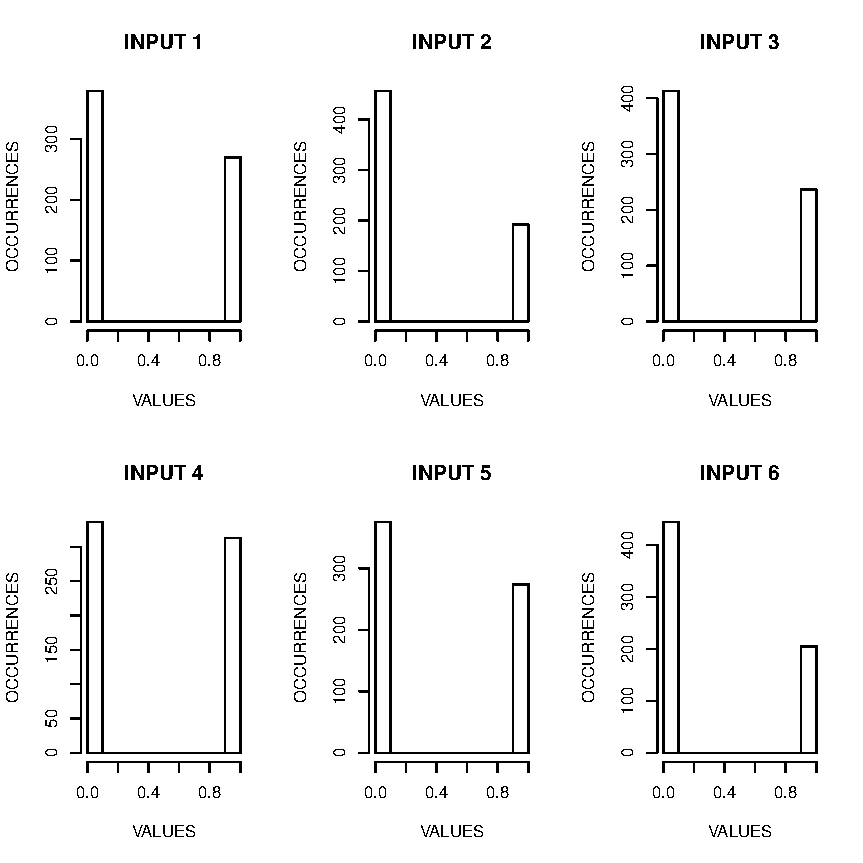
\includegraphics[width=\columnwidth]{images/input1_6.pdf}
  \caption{First six input variables}
  \label{fig:input16}
\end{figure}

\begin{figure}[!h]
  \vspace{-0.2cm}
  \centering
  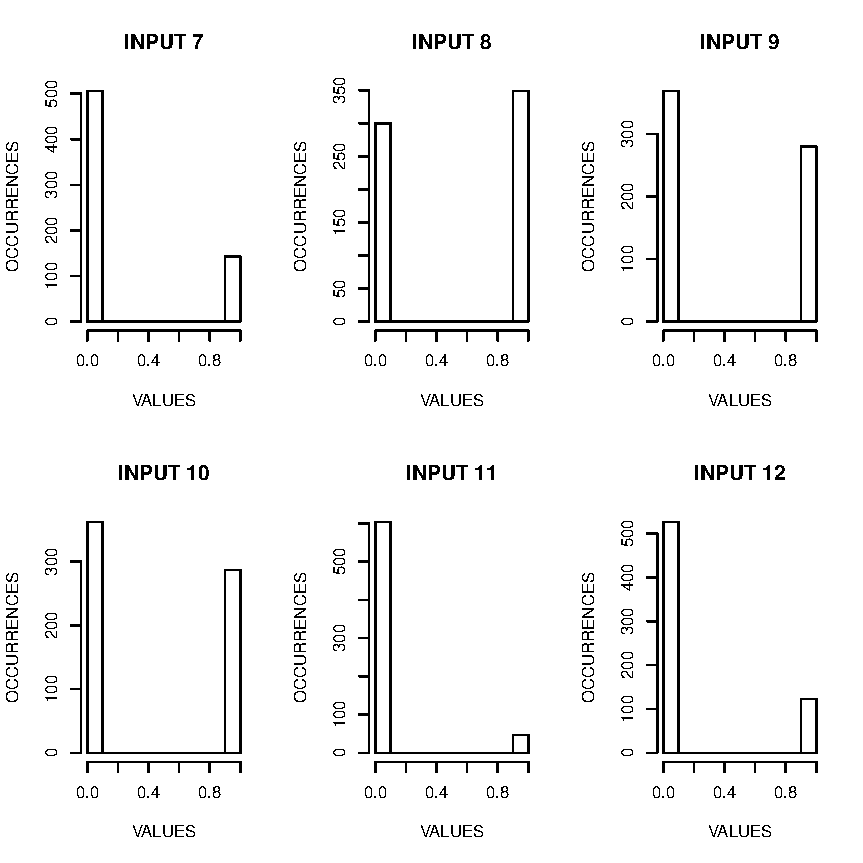
\includegraphics[width=\columnwidth]{images/input7_12.pdf}
  \caption{Last six input variables}
  \label{fig:input712}
\end{figure}

Figure \ref{fig:impacthistogram} presents gamma normalized real outcome from PERIL in a histogram. A shape of the distribution fitting function is also presented in a curve under the histogram.

\begin{figure}[!h]
  \vspace{-0.2cm}
  \centering
  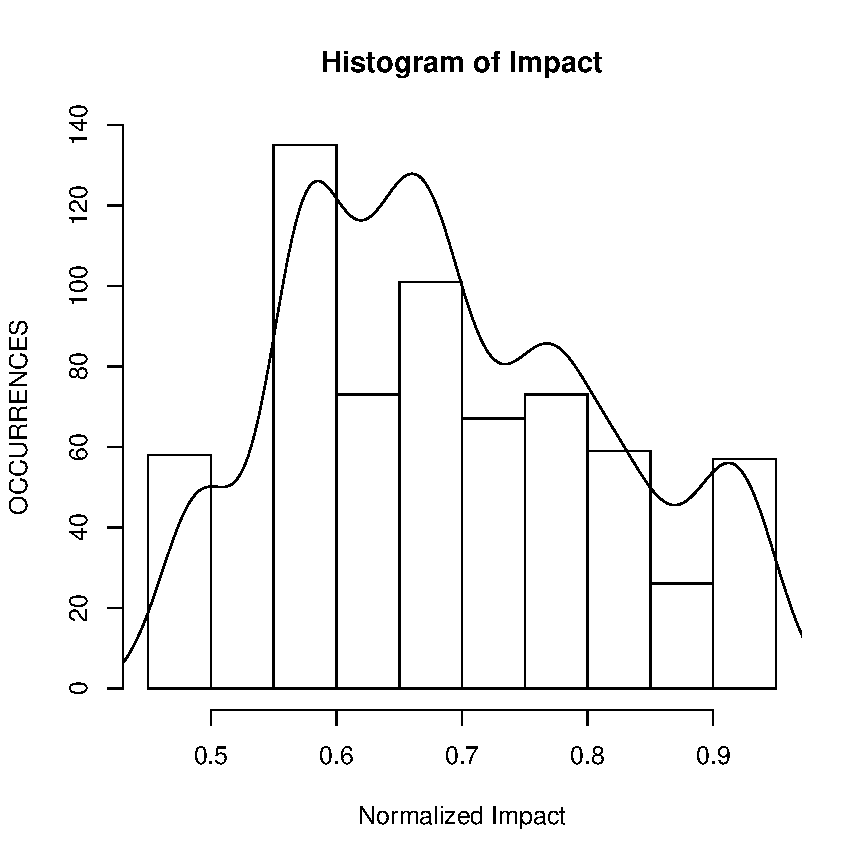
\includegraphics[width=\columnwidth]{images/impact_histogram.pdf}
  \caption{Histogram of impact and shape of the distribution fitting function}
  \label{fig:impacthistogram}
\end{figure}

\subsection{Tools}
\label{sec:tools}

\noindent Monte Carlo Simulation was performed in Microsoft Office Excel. Data Analysis complement was utilized to obtain random values from customized sample. R language is a programming language and an environment for statistical computing, data manipulation, calculation and graphical display \cite{venables2002introduction}. R was utilized to conduct experiments with Multiple Linear Regression (MLR) and Regression Tree Model (RTM). The MultiLayer Perceptron (MLP) model used in this analysis was developed in Java. The source code implements data preprocessing, training, cross-validation, testing and MAE evaluation. It was based on \cite{valenca2005aplicando} book. We have utilized WEKA API \cite{hall2009weka} to program SVM. The built-in implementation of SVM is SMOreg. \cite{Smola1998} proposed an iterative algorithm, called sequential minimal optimization (SMO), for solving the regression problem using SVM. SMOreg is a SMO program. SMOreg come across our needs, because the regression model could be generated after testing and cross-validation as stopping criteria.
% Apresentar a ferramenta Weka e como elas foram configuradas.
%The Waikato Environment for Knowledge Analysis (WEKA) \cite{hall2009weka} came about through the perceived need for a unified workbench that would allow researchers easy access to state of the art techniques in machine learning. WEKA project allows users to quickly try out and compare different machine learning methods on new datasets. Its modular and extensible architecture allows sophisticated data mining processes to be built up from the wide collection of base learning algorithms and tools provided. Extend the toolkit is easy because of a simple API, plugin mechanisms and facilities that automate the integration of new learning algorithms with WEKA’s graphical user interfaces \cite{hall2009weka}.

\subsection{Experiment}
\label{sec:experiment}

% Descrever os parâmetros de cada algoritmo utilizado.
\noindent Monte Carlo Simulation used the entire dataset. In order to increase the performance prediction, we have filtered only the possible real outcomes to generate the calculated outcome. Towards this decision, we reduce generalization problems and improve MCS performance.

In this study, the source code of MLR model was adapted from Torgo \cite{torgo2003data}, in order to perform linear regression model training, cross-validation, outcome prediction and MAE evaluation. MRLM and Regression Tree Model (RTM) methods were analyzed statistically to define the baseline linear regression model for further analysis. The results for this previous analysis are also presented in Section \ref{sec:resultanalysis}.

% Descrever os parametros da MLP
A three layered back-propagation MLP model was established to model risk impact prediction mechanism. The MLP model consisted of one input layer, one hidden layer, and one output layer. The input layer had thirteen neurons, which represent the twelve independent variables plus the bias. The output layer has one neuron, which represents the single impact outcome. The number of neurons in the hidden layer was determined by trial and error to achieve more accurate performance of MLP model. The transfer functions of hidden and output layer was sigmoid-logistic. The architecture of the MLP model is demonstrated in Figure \ref{fig:mlpmodelstudy}.

\begin{figure}[!h]
  \vspace{-0.2cm}
  \centering
  \def \svgwidth{\columnwidth}
  \input{images/mlp.pdf_tex}
  \caption{MLP model utilized in the study.}
  \label{fig:mlpmodelstudy}
\end{figure}

For our purpose, PERIL was split into three disjoint subsets - training, cross-validation and test subset, corresponding to fifty percent, twenty-five percent and twenty five percent of the dataset, respectively. The \textit{early stopping} method and the \textit{split-sample} cross-validation method were combined and used for ANN training \cite{priddy2005artificial}.

The maximum training epochs has been set at six hundreds. Starting with one neuron in the hidden layer, the MLP model was trained and tested. Each time, the number of neurons was increased by one, until reach ten, from which the number of neurons was increased by ten. The maximum number of neurons in hidden layer was one hundred. Accordingly, the best found MLP structure was established. 

Learning rate, momentum and hidden neurons varied from values are presented in Table \ref{tab:mlp_configuration_investigation}. A better parameters configuration investigated is shown in Table \ref{tab:mlp_best_configuration}. Figure \ref{fig:mlpmodelstudy} presents the MLP model with better configuration for PERIL. The model contains ten neurons in hidden layer.

\begin{table}[h]
\caption{Parameters intervals to MLP model.}\label{tab:mlp_configuration_investigation} \centering
\begin{tabular}{|c|c|c|}
  \hline
  Parameter & Min. Value & Max. Value \\
  \hline
  Momentum & 0.5 & 0.9 \\
  \hline
  Learning rate & 0.1 & 0.5 \\
  \hline
  Hidden Neurons & 1 & 100 \\
  \hline
\end{tabular}
\end{table}

\begin{table}[h]
\caption{A better parameters configuration to MLP model.}\label{tab:mlp_best_configuration} \centering
\begin{tabular}{|c|c|}
  \hline
  Parameter & Value \\
  \hline
  Momentum & 0.5 \\
  \hline
  Learning rate & 0.1 \\
  \hline
  Hidden Neurons & 10 \\
  \hline
  Maximum Cycles & 600 \\
  \hline
\end{tabular}
\end{table}

% Descrever a SVM utilizada e seus parâmetros
According to our analysis requirement, PERIL was also partitioned into three disjoint subsets to be used with SVM - training, cross-validation and test subset, using the same percentage utilized in MLP. In SVM source code, RegSMOImproved is the optimization algorithm and PolyKernel is the kernel function as described in \cite{Shevade1999}. 
%\begin{small}
%\label{code:svm}
%\begin{verbatim}
% Begin
%     peril <- read_file();
%     peril_train <- partition(peril, 0, 50);
%     peril_crossvalidation <- partition(peril, 50, 75);
%     peril_test <- partition(peril, 75, 100);
%     smo <- SMOReg();
%     options <- [peril_train, peril_crossvalidation, 
%                 RegSMOImproved, PolyKernel]
%     SMOReg.runClassifier(smo, options);
%     for instance in peril_test:
%          calculated <- smo.classifyInstance(instance);
%          wished <- instance.classValue();
%          MAE <- MAE + absolute(wished - calculated)
%     end
%     n <- peril_test.size();
%     MAE <- MAE/n;
% End
%\end{verbatim}
%\end{small}
%In Algorithm \ref{code:svm}, we read data on file, split data into training, cross-validation and testing subsets, instantiates SMOReg SVM regression model, run model training, generates a calculated outcome, get the correspondent real output in PERIL and calculate MAE.

\section{\uppercase{Result Analysis}}
\label{sec:resultanalysis}

%Apresentar os resultados lado a lado para cada algoritmo:
% 1. Apresentar a estatística descritiva para os resultados obtidos dos experimentos (esperado e o obtido).
% 2. Apresentar o erro médio absoluto para as estimatívas.
\noindent Initially, the previous analysis consists of choosing between MLRM and RTM as baseline for the next analysis. It could be performed after discussing the information provided in Table \ref{tab:lm_descriptive} and in Figure \ref{fig:mlrm_result}. 

Table \ref{tab:lm_descriptive} shows descriptive statistics of normalized MAE's to both algorithms. Average, standard deviation, minimum and maximum value are calculated for MLRM (cv.lm.v1), $RTM_1$ (cv.rpart.v1), $RTM_2$ (cv.rpart.v2) and $RTM_3$ (cv.rpart.v3). $RTM_1$, $RTM_2$ and $RTM_3$ are regression tree models instances automatically generated by R in this analysis. MLRM has minor values for all statistics.

\begin{table}[h]
\caption{Descriptive statistics for normalized errors of linear regression models.}\label{tab:lm_descriptive} \centering
\begin{tabular}{|c|c|c|c|c|}
  \hline
   & MLRM & $RTM_1$ & $RTM_2$ & $RTM_3$ \\
  \hline
  Average & \textbf{0.09912} & 0.10238 & 0.10305 & 0.10361  \\
  \hline
  Std Dev & \textbf{0.00391} & 0.00423 & 0.00441 & 0.00426  \\
  \hline
  Min. & \textbf{0.08956} & 0.09214 & 0.09321 & 0.09372  \\
  \hline
  Max. & \textbf{0.10746} & 0.11231 & 0.11267 & 0.11359  \\
  \hline
\end{tabular}
\end{table}

\begin{figure}[!h]
  \vspace{-0.2cm}
  \centering
  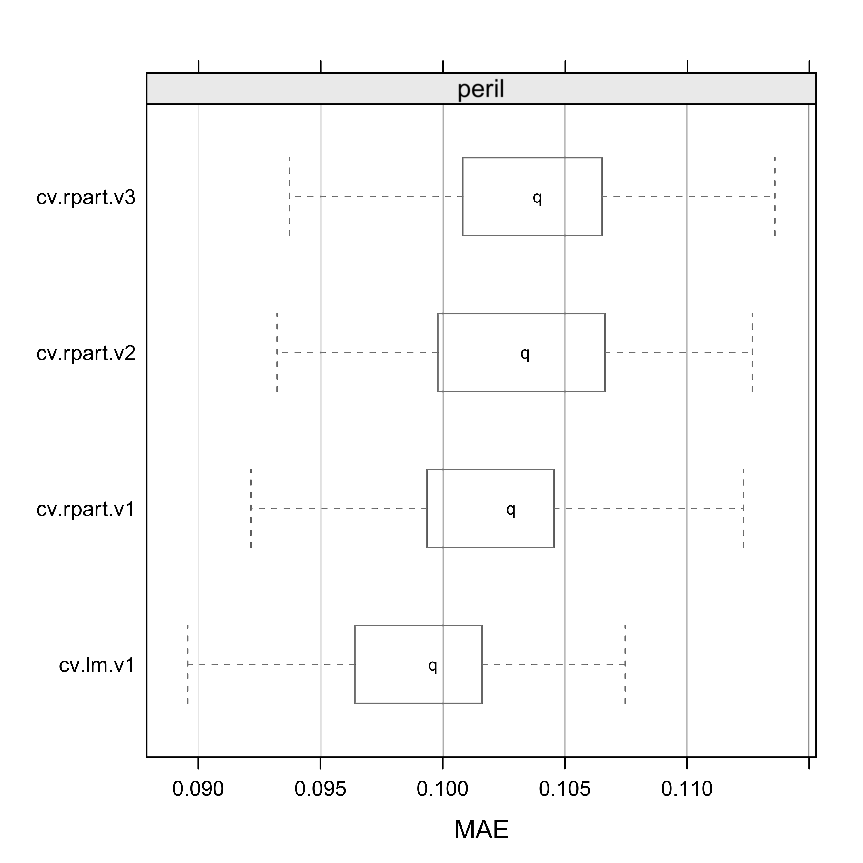
\includegraphics[width=\columnwidth]{images/mlrm_result_peril.pdf}
  \caption{Boxplots for normalized errors of linear regression models.}
  \label{fig:mlrm_result}
\end{figure}

In Figure \ref{fig:mlrm_result}, normalized MAE's boxplots after predictions for $RTM_3$, $RTM_2$, $RTM_1$ and MLRM are presented. The minor MAE is obtained on MLRM, this regression model also has minor standard deviation. From those information, we can affirm MLRM is a more efficient and precise model and will be introduced in the experiment as baseline method.

Finally, normalized MAE's of selected approaches for the experiment, described in Subsection \ref{sec:experiment}, are analyzed towards information presented in Table \ref{tab:final_descriptive} and Figure \ref{fig:final_result}. 

Table \ref{tab:final_descriptive} shows descriptive statistics of normalized MAE's for each approach. It was perceived that SVM has	lower values for minimum (Min.), median, mean and maximum (Max.) errors. Nevertheless, MLP has minor standard deviation (Std.) value.

\begin{table}[h]
\caption{Descriptive statistics for SVM, MLP, MLR and MCS.}\label{tab:final_descriptive} \centering
\begin{tabular}{|c|c|c|c|c|}
  \hline
   & SVM & MLP & MLR & MCS \\
  \hline
  Min. & \textbf{0.08347} & 0.09736 & 0.09764 & 0.10410  \\
  \hline
  Median & \textbf{0.09374} & 0.10014 & 0.10798 & 0.12740 \\
  \hline
  Mean & \textbf{0.09430} & 0.10005 & 0.10798 & 0.12640 \\
  \hline
  Std. & 0.00488 & \textbf{0.00154} & 0.00794 & 0.01250 \\
  \hline
  Max. & \textbf{0.10284} & 0.10413 & 0.12927 & 0.14950 \\
  \hline
\end{tabular}
\end{table}

In Figure \ref{fig:final_result}, it is observed that the traditional technique, MCS (MonteCarlo), has a large standard deviation. It is due to randomness in MCS method, one of its limitation. Besides that, MCS has higher results in descriptive statistics. On the other hand, comparing MCS with MLR outcomes, it is noticed that MLR has better statistical values. Thus, we could not identify a reason to justify MCS usage as proposed by \cite{PMBOK2008}.

Besides that, MLP seems to be a promising alternative because it is such a optimized MLR. In this analysis, it is a more precise method to risk impact estimation. Since MLP can be interpreted as a non-linear regression model, it must provide more valuable results than MLR.

Lastly, SVM is a more efficient approach because it explores minor results, but less precise than MLP. It has a good generalization capability such as MLP, since its inter-quartil interval is the second shorter. But above all, SVM could explore MAE minimization. We can realize it looking at Figure \ref{fig:svm_exclusive}, where the most of values are near and above median value. Therefore, accordingly with this experiment, SVM seems to be a more accurate method to risk impact estimation using PERIL.

\begin{figure}[!h]
  \vspace{-0.2cm}
  \centering
  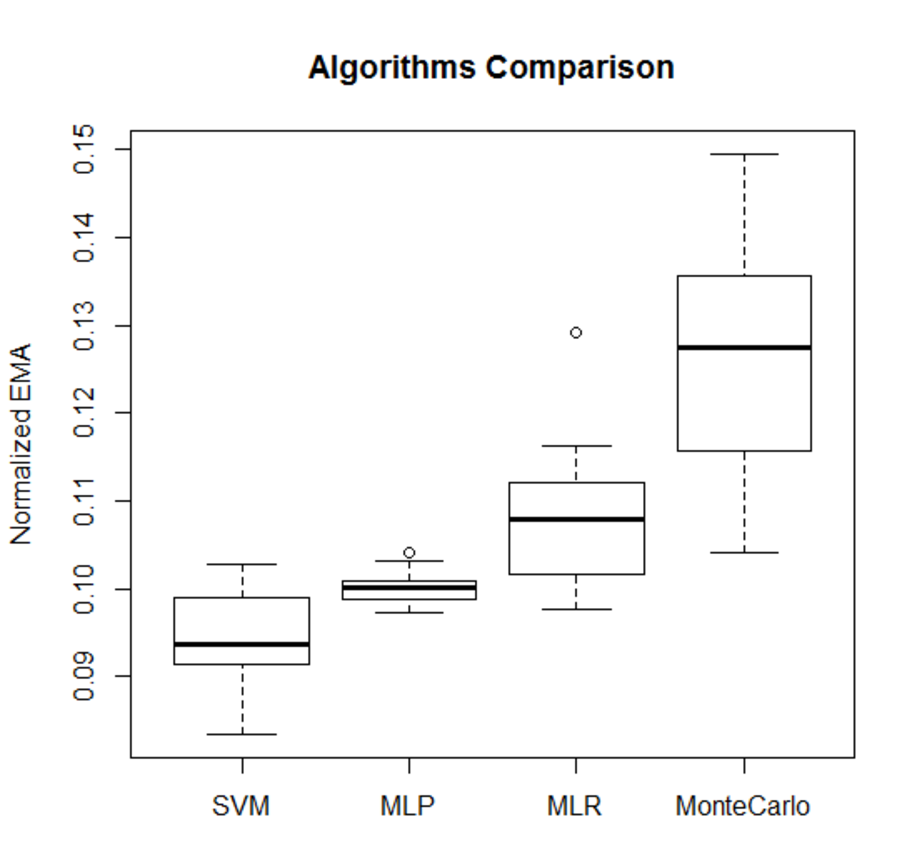
\includegraphics[width=\columnwidth]{images/resul_final.pdf}
  \caption{Boxplots of analyzed methods.}
  \label{fig:final_result}
\end{figure}

\begin{figure}[!h]
  \vspace{-0.2cm}
  \centering
  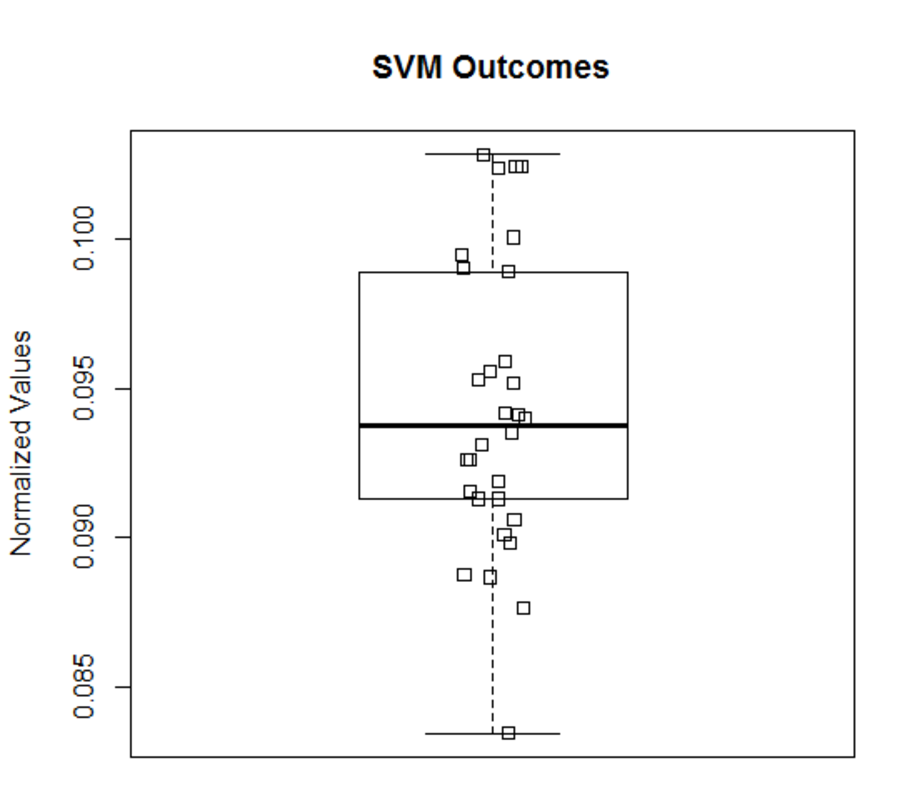
\includegraphics[width=\columnwidth]{images/svm_exclusive.pdf}
  \caption{SVM boxplot with individual values.}
  \label{fig:svm_exclusive}
\end{figure}

\section{\uppercase{Conclusion}}
\label{sec:conclusion}

\noindent This paper has investigated the use of Artificial Neural Networks algorithms, like SVM and MLP, for estimation of risk impact in software project risk analysis. We have carried out a statistical analysis using PERIL. The results were compared to MLRM and Monte Carlo Simulation, a traditional approach proposed by \cite{PMBOK2008}. We have considered improving risk impact estimation accuracy during software project management, in terms of MAE mean and standard deviation. We have observed that MLP had minor standard deviation estimation error, and showed to be a promissory technique. Moreover, SVM had minor estimation error outcomes using PERIL. Therefore, the selected ANN algorithms outperformed both linear regression and MCS.
% Apresentar os melhores resultados obtidos.
% Apresentar as limitações desse estudo e trabalhos futuros.

\section*{\uppercase{Acknowledgements}}

\noindent The authors would like to thank Gildo Dantas and Rodrigo Lira for their notable contribution and incentives during this work. Finally, the authors would like to sincerely thank Professor Tom Kendrick for his generosity in providing PERIL to this study.

\bibliographystyle{apalike}
{\small
\bibliography{example}}
%\section*{\uppercase{Appendix}}
%\noindent If any, the appendix should appear directly after the
%references without numbering, and not on a new page. To do so please use the following command:
%\textit{$\backslash$section*\{APPENDIX\}}

\vfill

\end{document}

